\section{Definitions and Observations}
\label{sec:Definitions and Observations}
\subsection{Graphs and Paths}
\label{sub:Graphs and Paths}
We start by writing out some basic definitions from graph theory.
\begin{definition}
  A \textbf{graph} $\bm{G} = (G, N)$ is a tuple where the first element $G$ is a set representing the nodes in the graph, while the second element $N$ is a set representing the edges (neighbours).
  $N$ is usually represented as a subset of $G \times G$ where $(u,v) \in N$ iff there is an edge from node $u$ to node $v$ in the graph.
\end{definition}
Another way to think of $N$ is as a function $N: G \rightarrow \mathcal{P}(G)$ where $N(x)$ returns the set of all out-neighbours of $x$.
\begin{definition}
  A \textbf{path} is a sequence of nodes $(x_0, x_1, x_2, \dots, x_n)$ from the graph in which all nodes (except possibly the first and last) are distinct, such that for any two consequtive nodes $x_i,x_{i+1}$, we have that $(x_i, x_{i+1}) \in N$.
  In this case we say that there is a path from $x_0$ to $x_n$.
\end{definition}
For every $x$ in the graph, we have the unique empty path $(x)$ of length 0.
This path is distinct from the loop $(x,x)$.
\subsection{Proof-specific relations}
\label{sub:Proof-specific relations}
\begin{definition}
  Given a node $x$ and a collection of nodes $Y$, we have that \bm{$E(x,Y)$} holds iff $x$ has outgoing edges targeting exactly the nodes in $Y$\todo{This definition has to be changed}.
\end{definition}
\begin{definition}
  Given two nodes $x,y$ we have that \bm{$P(x,y)$} holds iff there exists a path between $x$ and $y$.
  We will use \bm{$P_o$} and \bm{$P_e$} to denote paths of odd and even lengths, respectively.
\end{definition}
The text will sometimes use the notion of \textit{path lengths}.  This will not refer to the actual length of the path, but whether or not it is of even or odd length.
\begin{definition}
  A path $P(x_0,x_n)$ is \textbf{fully trimmed} (denoted \bm{$P^f(x_0,x_n)$}) if no nodes in the path branches off elsewhere.
  This means that for every pair of consecutive nodes $x_i,x_{i+1}$ in the path, we need that $E(x_i,\{ x_{i+1} \})$.
\end{definition}
\begin{definition}
  A path $P(x_0,x_n)$ is \textbf{evenly trimmed} (denoted \bm{$P^e(x_0,x_n)$}) if every evenly indexed node is non-branching.
  Said differently, for every \textit{even} $i < n$ we need $E(x_i,\{x_{i+1}\})$ to hold.
\end{definition}
\begin{definition}
  A path $P(x_0,x_n)$ is \textbf{oddly trimmed} (denoted \bm{$P^o(x_0,x_n)$}) if for every \textit{odd} $i < n$, $E(x_i,\{x_{i+1}\})$ holds.
\end{definition}
We will usually denote paths with both length and trim in combination, i.e. $\peo(x,y)$.
This is solely to simplify the proofs and is nothing more than an abbreviation for $P^e(x,y) \wedge P_o(x,y)$, meaning an evenly trimmed odd path from $x$ to $y$.
\begin{definition}
  There is a \textbf{vel} between two nodes $x$ and $y$ (denoted \bm{$V(x,y)$}) if and only if there exists a node $c$ such that $P^o(x,c)$ and $P^o(y,c)$ and the sum of the two path lengths is odd. In formal terms we have that
  \[
  V(x,y) \Leftrightarrow (\poo(x,c) \wedge \poe(y,c)) \vee (\poe(x,c) \wedge \poo(y,c))
  \]
\end{definition}
By introducing a bit more notation, we will be able to write this formal defintion of a vel in a nicer way.
By generalizing over the actual lengths and trims of paths we can make statements like:
\[P_x(a,b) \wedge P_x(b,c) \Rightarrow P_e(a,c) \quad\text{where}\quad x \in \{e,o\}\]
This lets us argue about paths of equal length (even or odd) in one statement instead of explicitly describing both cases.
The statements above tells us that the concatenation of two paths of equal length (even or odd) results in an even path\todo{Rewrite section. Use P+E examples instead of P+P}.

Similarly, we can argue about paths of different lengths by introducing $\overline{x}$ as a piece of notation such that $\overline{o} = e$ and $\overline{e} = o$.
We can now make statements like \[P_x(a,b) \wedge P_{\overline{x}}(b,c) \Rightarrow P_o(a,c)\] telling us that concatenating two paths of different lengths (even or odd) results in an odd path.
We are now able to write our definition of a vel in a nice, shorter way\todo{Does the definition below need an existencial quantifier?}:
\[
V(a,b) \Leftrightarrow \exists x(\pox(a,c) \wedge \ponx(b,c))
\]
\subsection{Immediate observations}
\label{sub:Immediate observations}
\begin{lemma}
  $P^f(x,y) \Rightarrow P^o(x,y) \wedge P^e(x,y)$
\end{lemma}
 This implication should be easy to accept; a fully trimmed path has branching restrictions on all its nodes, both the odd and the even ones.
 It is thus both oddly and evenly trimmed.

 The opposite implication is actually also true, allthough not as obvious, since it would seem that $P^o(x,y)$ could refer to a path partly disjoint from $P^e(x,y)$ and there would thus be no single path both oddly and evenly trimmed.
 We will later show that this can't actually be the case.
\begin{lemma}
  $P_e(x,x)$ for every $x \in G_v$
\end{lemma}
This will denote the empty path mentioned earlier.
The path is even simply because 0 is even.
\begin{lemma}
  $E(x,\{ y \}) \Rightarrow P^f_o(x,y)$
\end{lemma}
An edge is another trivial example of a path.
The path is fully trimmed since $x$ does not branch off.
In the more general case of $E(x,Y)$, we have that $P^o_o(x,y)$ holds for every $y \in Y$.
\begin{lemma}
  $\poo(x,y) \Rightarrow V(x,y)$
\end{lemma}
A vel needs two paths of even and odd length, respectively.
Since the even path can be empty, we get that any odd path is a vel by itself.
\section{Path composition}
\label{sec:Path composition}
Suppose we have two paths; one from $a$ to $b$ and one from $b$ to $c$.
We can now obtain\todo{We don't really create anything here.  Is \textit{have} a better wording?} a path going from $a$ to $c$ by first traversing from $a$ to $b$ using the first path, then traversing from $b$ to $c$ using the second path.
This operation is called \textbf{path composition} and the resulting path is called a \textbf{composite path}.
Our notation captures the concept of path composition in the following way:
\[
P(a,b) \wedge P(b,c) \Rightarrow P(a,c)
\]
In this case, we say that $P(a,b)$ is composed with $P(b,c)$.

Let's extend this statement in order to describe the change in length.
We observe that when composing two even -- or two odd -- paths, the resulting path will always be even, while composing one path of even length with one of odd length, the resulting path will be odd.
Introducing length to the equation thus gives us two cases:
\begin{align*}
  P_x(a,b) \wedge P_x(b,c) \Rightarrow P_e(a,c)\\
  P_x(a,b) \wedge P_{\overline{x}}(b,c) \Rightarrow P_o(a,c)
\end{align*}
The next step will be to extend these statements even further to also capture the behavior of trimming under composition.
In order to do this, let's first make some observations:

First, unlike with the length property, we do not have any guarantee that a composite path has a trim at all.
We might need to set certain restrictions to our two original paths in order to get a properly trimmed (either evenly or oddly) path as a result after composition.  It should at least be obvious that both original paths should be trimmed in some way.

Secondly, no matter what path you compose a trimmed path with, the resulting composite path will always be of the same trim, if trimmed at all.
This means that given a path $P^e(a,b)$ and a path $P(b,c)$, the composite path from $a$ to $c$ will never be oddly trimmed. Equivalently, a composition of $P^o(a,b)$ and $P(b,c)$ will never result in $P^e(a,c)$.

Now, let's look at some examples.
The below figure shows instances of the four possible combinations of trims and lengths of a path.
All nodes $x$ and edges $(x,y)$ such that $E(x,\{ y\})$ are depicted in red\todo{Should I avoid using colors in the paper?} and will from here on be referred to as \textit{non-branching} nodes and \textit{unique} edges, respectively\todo{Overkill?}.
\[
  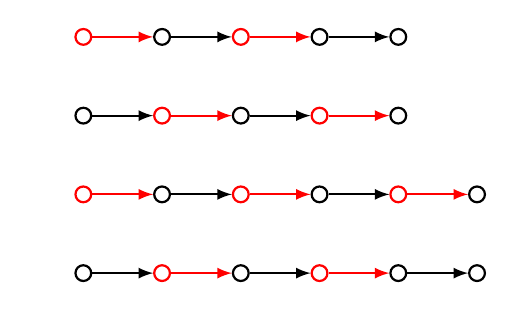
\begin{tikzpicture}
    [
    point/.style={thick,circle,draw,inner sep=0pt,minimum size=2mm},
    trimmed/.style={thick,draw=red},
    untrimmed/.style={thick,draw=black}
    ]
    \node (0) at (0,0) [point,label=left:$\poo\quad$] {};
    \node (1) at (1,0) [point,trimmed] {};
    \node (2) at (2,0) [point] {};
    \node (3) at (3,0) [point,trimmed] {};
    \node (4) at (4,0) [point] {};
    \node (5) at (5,0) [point] {};
    \draw [-latex,untrimmed] (0) to (1);
    \draw [-latex,trimmed] (1) to (2);
    \draw [-latex,untrimmed] (2) to (3);
    \draw [-latex,trimmed] (3) to (4);
    \draw [-latex,untrimmed] (4) to (5);

    \node (0) at (0,1) [point,trimmed,label=left:$\peo\quad$] {};
    \node (1) at (1,1) [point] {};
    \node (2) at (2,1) [point,trimmed] {};
    \node (3) at (3,1) [point] {};
    \node (4) at (4,1) [point,trimmed] {};
    \node (5) at (5,1) [point] {};
    \draw [-latex,trimmed] (0) to (1);
    \draw [-latex,untrimmed] (1) to (2);
    \draw [-latex,trimmed] (2) to (3);
    \draw [-latex,untrimmed] (3) to (4);
    \draw [-latex,trimmed] (4) to (5);

    \node (0) at (0,2) [point,label=left:$\poe\quad$] {};
    \node (1) at (1,2) [point,trimmed] {};
    \node (2) at (2,2) [point] {};
    \node (3) at (3,2) [point,trimmed] {};
    \node (4) at (4,2) [point] {};
    \draw [-latex,untrimmed] (0) to (1);
    \draw [-latex,trimmed] (1) to (2);
    \draw [-latex,untrimmed] (2) to (3);
    \draw [-latex,trimmed] (3) to (4);

    \node (0) at (0,3) [point,trimmed,label=left:$\pee\quad$] {};
    \node (1) at (1,3) [point] {};
    \node (2) at (2,3) [point,trimmed] {};
    \node (3) at (3,3) [point] {};
    \node (4) at (4,3) [point] {};
    \draw [-latex,trimmed] (0) to (1);
    \draw [-latex,untrimmed] (1) to (2);
    \draw [-latex,trimmed] (2) to (3);
    \draw [-latex,untrimmed] (3) to (4);
  \end{tikzpicture}
\]
Now comes the question:
What kind of paths can we put at the end of each of these different paths such that the resulting composite path would be properly trimmed (either evenly or oddly)?

Let us start by looking at evenly trimmed even paths ($\pee$).
The first edge in a path of this type is obviously always unique, but since the path is of even length, we also know that its \textit{last} edge does not have this uniqueness property. In order to preserve the even trim under composition, the first edge of the consecutive path therefore has to be unique.
This means that given $\pee(a,b)$ and $P(b,c)$, the composite path is evenly trimmed only when $P(b,c)$ is evenly trimmed.

The following figures examplifies this:
\[
  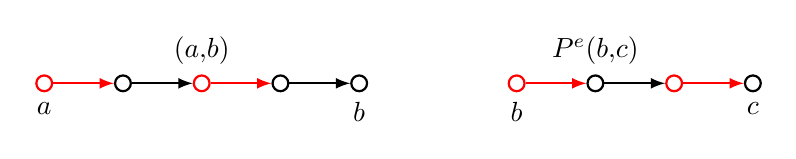
\begin{tikzpicture}
    [
    point/.style={thick,circle,draw,inner sep=0pt,minimum size=2mm},
    trimmed/.style={thick,draw=red},
    untrimmed/.style={thick,draw=black}
    ]
    \node (0) at (0,0) [point,trimmed,label=below:$a$] {};
    \node (1) at (1,0) [point] {};
    \node (2) at (2,0) [point,trimmed,label=above:$\pee(a{,}b)$] {};
    \node (3) at (3,0) [point] {};
    \node (4) at (4,0) [point,label=below:$b$] {};
    \node (5) at (6,0) [point,trimmed,label=below:$b$] {};
    \node (6) at (7,0) [point,label=above:$P^e(b{,}c)$] {};
    \node (7) at (8,0) [point,trimmed] {};
    \node (8) at (9,0) [point,label=below:$c$] {};
    \draw [-latex,trimmed] (0) to (1);
    \draw [-latex,untrimmed] (1) to (2);
    \draw [-latex,trimmed] (2) to (3);
    \draw [-latex,untrimmed] (3) to (4);
    \draw [-latex,trimmed] (5) to (6);
    \draw [-latex,untrimmed] (6) to (7);
    \draw [-latex,trimmed] (7) to (8);
  \end{tikzpicture}
\]

Composing the two paths above will give an evenly trimmed path from $a$ to $b$.
\[
  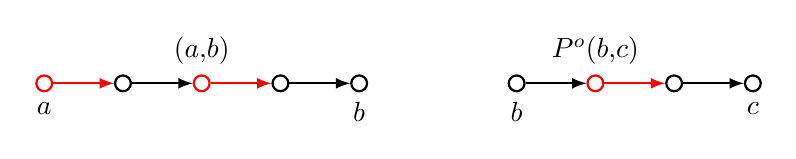
\begin{tikzpicture}
    [
    point/.style={thick,circle,draw,inner sep=0pt,minimum size=2mm},
    trimmed/.style={thick,draw=red},
    untrimmed/.style={thick,draw=black}
    ]
    \node (0) at (0,0) [point,trimmed,label=below:$a$] {};
    \node (1) at (1,0) [point] {};
    \node (2) at (2,0) [point,trimmed,label=above:$\pee(a{,}b)$] {};
    \node (3) at (3,0) [point] {};
    \node (4) at (4,0) [point,label=below:$b$] {};
    \node (5) at (6,0) [point,label=below:$b$] {};
    \node (6) at (7,0) [point,trimmed,label=above:$P^o(b{,}c)$] {};
    \node (7) at (8,0) [point] {};
    \node (8) at (9,0) [point,label=below:$c$] {};
    \draw [-latex,trimmed] (0) to (1);
    \draw [-latex,untrimmed] (1) to (2);
    \draw [-latex,trimmed] (2) to (3);
    \draw [-latex,untrimmed] (3) to (4);
    \draw [-latex,untrimmed] (5) to (6);
    \draw [-latex,trimmed] (6) to (7);
    \draw [-latex,untrimmed] (7) to (8);
  \end{tikzpicture}
\]

Composing the two paths above will \textit{not} give an evenly trimmed path from $a$ to $b$, since it will contain two consecutive edges without the uniqueness property.\\

The first thing to notice with these paths is that the last edges of $\poe$ and $\peo$ are both unique, while the last edges of $\pee$ and $\poo$ are not.
It should be clear that this property holds for all instances of these four path types\todo{Should this be further justified?}, not only the examples given above.  It should therefore suffice to show the properties using our example paths only.

Notice how the last edge of these paths is never unique (red).  This means that in order to preserve the even trim, the first edge of the consecutive path needs to be a unique one, i.e. the path has to be evenly trimmed.\todo{This section is not done.  I feel like I have already been talking too much about obvious concepts.}
